\documentclass[twoside]{book}

% Packages required by doxygen
\usepackage{fixltx2e}
\usepackage{calc}
\usepackage{doxygen}
\usepackage[export]{adjustbox} % also loads graphicx
\usepackage{graphicx}
\usepackage[utf8]{inputenc}
\usepackage{makeidx}
\usepackage{multicol}
\usepackage{multirow}
\PassOptionsToPackage{warn}{textcomp}
\usepackage{textcomp}
\usepackage[nointegrals]{wasysym}
\usepackage[table]{xcolor}

% Font selection
\usepackage[T1]{fontenc}
\usepackage[scaled=.90]{helvet}
\usepackage{courier}
\usepackage{amssymb}
\usepackage{sectsty}
\renewcommand{\familydefault}{\sfdefault}
\allsectionsfont{%
  \fontseries{bc}\selectfont%
  \color{darkgray}%
}
\renewcommand{\DoxyLabelFont}{%
  \fontseries{bc}\selectfont%
  \color{darkgray}%
}
\newcommand{\+}{\discretionary{\mbox{\scriptsize$\hookleftarrow$}}{}{}}

% Page & text layout
\usepackage{geometry}
\geometry{%
  a4paper,%
  top=2.5cm,%
  bottom=2.5cm,%
  left=2.5cm,%
  right=2.5cm%
}
\tolerance=750
\hfuzz=15pt
\hbadness=750
\setlength{\emergencystretch}{15pt}
\setlength{\parindent}{0cm}
\setlength{\parskip}{3ex plus 2ex minus 2ex}
\makeatletter
\renewcommand{\paragraph}{%
  \@startsection{paragraph}{4}{0ex}{-1.0ex}{1.0ex}{%
    \normalfont\normalsize\bfseries\SS@parafont%
  }%
}
\renewcommand{\subparagraph}{%
  \@startsection{subparagraph}{5}{0ex}{-1.0ex}{1.0ex}{%
    \normalfont\normalsize\bfseries\SS@subparafont%
  }%
}
\makeatother

% Headers & footers
\usepackage{fancyhdr}
\pagestyle{fancyplain}
\fancyhead[LE]{\fancyplain{}{\bfseries\thepage}}
\fancyhead[CE]{\fancyplain{}{}}
\fancyhead[RE]{\fancyplain{}{\bfseries\leftmark}}
\fancyhead[LO]{\fancyplain{}{\bfseries\rightmark}}
\fancyhead[CO]{\fancyplain{}{}}
\fancyhead[RO]{\fancyplain{}{\bfseries\thepage}}
\fancyfoot[LE]{\fancyplain{}{}}
\fancyfoot[CE]{\fancyplain{}{}}
\fancyfoot[RE]{\fancyplain{}{\bfseries\scriptsize Generated by Doxygen }}
\fancyfoot[LO]{\fancyplain{}{\bfseries\scriptsize Generated by Doxygen }}
\fancyfoot[CO]{\fancyplain{}{}}
\fancyfoot[RO]{\fancyplain{}{}}
\renewcommand{\footrulewidth}{0.4pt}
\renewcommand{\chaptermark}[1]{%
  \markboth{#1}{}%
}
\renewcommand{\sectionmark}[1]{%
  \markright{\thesection\ #1}%
}

% Indices & bibliography
\usepackage{natbib}
\usepackage[titles]{tocloft}
\setcounter{tocdepth}{3}
\setcounter{secnumdepth}{5}
\makeindex

% Hyperlinks (required, but should be loaded last)
\usepackage{ifpdf}
\ifpdf
  \usepackage[pdftex,pagebackref=true]{hyperref}
\else
  \usepackage[ps2pdf,pagebackref=true]{hyperref}
\fi
\hypersetup{%
  colorlinks=true,%
  linkcolor=blue,%
  citecolor=blue,%
  unicode%
}

% Custom commands
\newcommand{\clearemptydoublepage}{%
  \newpage{\pagestyle{empty}\cleardoublepage}%
}

\usepackage{caption}
\captionsetup{labelsep=space,justification=centering,font={bf},singlelinecheck=off,skip=4pt,position=top}

%===== C O N T E N T S =====

\begin{document}

% Titlepage & ToC
\hypersetup{pageanchor=false,
             bookmarksnumbered=true,
             pdfencoding=unicode
            }
\pagenumbering{alph}
\begin{titlepage}
\vspace*{7cm}
\begin{center}%
{\Large Coppelia\+Sim-\/\+Interface }\\
\vspace*{1cm}
{\large Generated by Doxygen 1.8.13}\\
\end{center}
\end{titlepage}
\clearemptydoublepage
\pagenumbering{roman}
\tableofcontents
\clearemptydoublepage
\pagenumbering{arabic}
\hypersetup{pageanchor=true}

%--- Begin generated contents ---
\chapter{Hierarchical Index}
\section{Class Hierarchy}
This inheritance list is sorted roughly, but not completely, alphabetically\+:\begin{DoxyCompactList}
\item Robot\+HW\begin{DoxyCompactList}
\item \contentsline{section}{coppeliasim\+\_\+interface\+:\+:Hardware\+Interface}{\pageref{classcoppeliasim__interface_1_1HardwareInterface}}{}
\end{DoxyCompactList}
\item \contentsline{section}{coppeliasim\+\_\+interface\+:\+:Simulation\+Synchronizer}{\pageref{classcoppeliasim__interface_1_1SimulationSynchronizer}}{}
\end{DoxyCompactList}

\chapter{Class Index}
\section{Class List}
Here are the classes, structs, unions and interfaces with brief descriptions\+:\begin{DoxyCompactList}
\item\contentsline{section}{\hyperlink{classcoppeliasim__interface_1_1HardwareInterface}{coppeliasim\+\_\+interface\+::\+Hardware\+Interface} \\*Hardware-\/\+Interface for the U\+R10e-\/model in Coppelia\+Sim that behaves just like the driver for the real robot }{\pageref{classcoppeliasim__interface_1_1HardwareInterface}}{}
\item\contentsline{section}{\hyperlink{classcoppeliasim__interface_1_1SimulationSynchronizer}{coppeliasim\+\_\+interface\+::\+Simulation\+Synchronizer} \\*Synchronizes the R\+O\+S-\/time with the Coppelia\+Sim-\/time in the sense, that both \textquotesingle{}clocks\textquotesingle{} are running at the same speed (but not necessarely at the same time), and ensures that time-\/critical tasks in the R\+O\+S-\/domain are performed in sync with each simulation-\/step }{\pageref{classcoppeliasim__interface_1_1SimulationSynchronizer}}{}
\end{DoxyCompactList}

\chapter{Class Documentation}
\hypertarget{classcoppeliasim__interface_1_1HardwareInterface}{}\section{coppeliasim\+\_\+interface\+:\+:Hardware\+Interface Class Reference}
\label{classcoppeliasim__interface_1_1HardwareInterface}\index{coppeliasim\+\_\+interface\+::\+Hardware\+Interface@{coppeliasim\+\_\+interface\+::\+Hardware\+Interface}}


Hardware-\/\+Interface for the U\+R10e-\/model in Coppelia\+Sim that behaves just like the driver for the real robot.  




{\ttfamily \#include $<$hardware\+\_\+interface.\+h$>$}



Inheritance diagram for coppeliasim\+\_\+interface\+:\+:Hardware\+Interface\+:\nopagebreak
\begin{figure}[H]
\begin{center}
\leavevmode
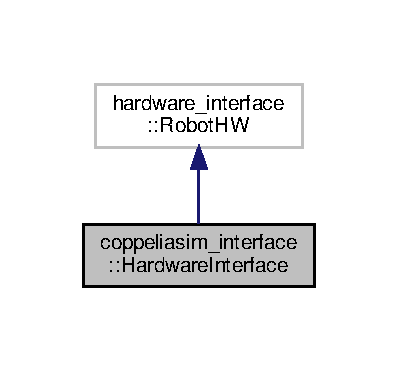
\includegraphics[width=191pt]{classcoppeliasim__interface_1_1HardwareInterface__inherit__graph}
\end{center}
\end{figure}


Collaboration diagram for coppeliasim\+\_\+interface\+:\+:Hardware\+Interface\+:\nopagebreak
\begin{figure}[H]
\begin{center}
\leavevmode
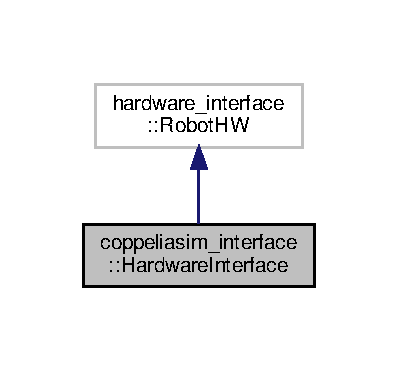
\includegraphics[width=191pt]{classcoppeliasim__interface_1_1HardwareInterface__coll__graph}
\end{center}
\end{figure}
\subsection*{Public Member Functions}
\begin{DoxyCompactItemize}
\item 
\mbox{\Hypertarget{classcoppeliasim__interface_1_1HardwareInterface_a731c52969b54a2cdda78a494bcd878ee}\label{classcoppeliasim__interface_1_1HardwareInterface_a731c52969b54a2cdda78a494bcd878ee}} 
\hyperlink{classcoppeliasim__interface_1_1HardwareInterface_a731c52969b54a2cdda78a494bcd878ee}{Hardware\+Interface} ()
\begin{DoxyCompactList}\small\item\em Construct a new Hardware Interface object and initialize all class members that do not require a R\+O\+S-\/ or Coppelia\+Sim-\/connection. \end{DoxyCompactList}\item 
\mbox{\Hypertarget{classcoppeliasim__interface_1_1HardwareInterface_a61047459c300ddd92e0b2d82e3b7c2e2}\label{classcoppeliasim__interface_1_1HardwareInterface_a61047459c300ddd92e0b2d82e3b7c2e2}} 
virtual \hyperlink{classcoppeliasim__interface_1_1HardwareInterface_a61047459c300ddd92e0b2d82e3b7c2e2}{$\sim$\+Hardware\+Interface} ()
\begin{DoxyCompactList}\small\item\em Destroy the Hardware Interface object and handle disconnection from Coppelia\+Sim. \end{DoxyCompactList}\item 
virtual bool \hyperlink{classcoppeliasim__interface_1_1HardwareInterface_ada54343beeb383c43951877e3d49cf8e}{init} (ros\+::\+Node\+Handle \&root\+\_\+nh, ros\+::\+Node\+Handle \&robot\+\_\+nh) override
\begin{DoxyCompactList}\small\item\em Connects program to Coppelia\+Sim and obtains the required handles. Reads in the required R\+O\+S-\/parameters and initializes all interfaces that are implemented in the real hardware-\/interface. \end{DoxyCompactList}\item 
virtual void \hyperlink{classcoppeliasim__interface_1_1HardwareInterface_abc05d9a9e8761462b2161a33f55203cc}{read} (const ros\+::\+Time \&, const ros\+::\+Duration \&) override
\begin{DoxyCompactList}\small\item\em Gets the joint-\/data (position, velocity, torque) from Coppelia\+Sim in a blocking way. \end{DoxyCompactList}\item 
\mbox{\Hypertarget{classcoppeliasim__interface_1_1HardwareInterface_a2a116645fc33233e4b9b1a37a9165674}\label{classcoppeliasim__interface_1_1HardwareInterface_a2a116645fc33233e4b9b1a37a9165674}} 
virtual void \hyperlink{classcoppeliasim__interface_1_1HardwareInterface_a2a116645fc33233e4b9b1a37a9165674}{write} (const ros\+::\+Time \&, const ros\+::\+Duration \&) override
\begin{DoxyCompactList}\small\item\em Set the joint-\/target-\/values (velocities or positions, depending on active controller) in Coppelia\+Sim in a blocking way. \end{DoxyCompactList}\item 
\mbox{\Hypertarget{classcoppeliasim__interface_1_1HardwareInterface_a5b7c2e8dcf2fa17ba6bde7ea001d59e3}\label{classcoppeliasim__interface_1_1HardwareInterface_a5b7c2e8dcf2fa17ba6bde7ea001d59e3}} 
virtual bool {\bfseries prepare\+Switch} (const std\+::list$<$ hardware\+\_\+interface\+::\+Controller\+Info $>$ \&start\+\_\+list, const std\+::list$<$ hardware\+\_\+interface\+::\+Controller\+Info $>$ \&stop\+\_\+list) override
\item 
virtual void \hyperlink{classcoppeliasim__interface_1_1HardwareInterface_aae36a63c5125172387cfcbf21f9a1c24}{do\+Switch} (const std\+::list$<$ hardware\+\_\+interface\+::\+Controller\+Info $>$ \&start\+\_\+list, const std\+::list$<$ hardware\+\_\+interface\+::\+Controller\+Info $>$ \&stop\+\_\+list) override
\begin{DoxyCompactList}\small\item\em Tries to turn on or off provided controllers. The provided controllers must be applicable with this \hyperlink{classcoppeliasim__interface_1_1HardwareInterface}{Hardware\+Interface}, otherwise they do not trigger any changes. \end{DoxyCompactList}\item 
bool \hyperlink{classcoppeliasim__interface_1_1HardwareInterface_af3204245bbf1e9e317d5d0a57b3c86c2}{zero\+F\+T\+Sensor} (std\+\_\+srvs\+::\+Trigger\+Request \&req, std\+\_\+srvs\+::\+Trigger\+Response \&res)
\begin{DoxyCompactList}\small\item\em Should normally tare the force-\/torque-\/sensor but is not implemented for performance reasons (service response gets delivered, but is always \textquotesingle{}success == false\textquotesingle{}) \end{DoxyCompactList}\item 
bool \hyperlink{classcoppeliasim__interface_1_1HardwareInterface_a0fb3b4bf382fc390db4d8c40036a683b}{set\+Speed\+Slider} (ur\+\_\+msgs\+::\+Set\+Speed\+Slider\+Fraction\+Request \&req, ur\+\_\+msgs\+::\+Set\+Speed\+Slider\+Fraction\+Response \&res)
\begin{DoxyCompactList}\small\item\em Sets the speed-\/scaling as requested. \end{DoxyCompactList}\item 
bool \hyperlink{classcoppeliasim__interface_1_1HardwareInterface_a00cc87162beaecdf82c1510ae84b2d95}{set\+Pause} (std\+\_\+srvs\+::\+Set\+Bool\+Request \&req, std\+\_\+srvs\+::\+Set\+Bool\+Response \&res)
\begin{DoxyCompactList}\small\item\em Controls if the robots running state (R\+U\+N\+N\+I\+NG = normal, P\+A\+U\+S\+ED = halted, R\+A\+M\+P\+UP = Accelerating from P\+A\+U\+S\+ED to R\+U\+N\+N\+I\+NG) \end{DoxyCompactList}\end{DoxyCompactItemize}
\subsection*{Protected Member Functions}
\begin{DoxyCompactItemize}
\item 
bool \hyperlink{classcoppeliasim__interface_1_1HardwareInterface_af95c41749882b5d60ba02695c6b51407}{check\+Controller\+Claims} (const std\+::set$<$ std\+::string $>$ \&claimed\+\_\+resources)
\begin{DoxyCompactList}\small\item\em Check if the \hyperlink{classcoppeliasim__interface_1_1HardwareInterface}{Hardware\+Interface} can command the joined named in claimed\+\_\+resources. \end{DoxyCompactList}\end{DoxyCompactItemize}


\subsection{Detailed Description}
Hardware-\/\+Interface for the U\+R10e-\/model in Coppelia\+Sim that behaves just like the driver for the real robot. 

\subsection{Member Function Documentation}
\mbox{\Hypertarget{classcoppeliasim__interface_1_1HardwareInterface_af95c41749882b5d60ba02695c6b51407}\label{classcoppeliasim__interface_1_1HardwareInterface_af95c41749882b5d60ba02695c6b51407}} 
\index{coppeliasim\+\_\+interface\+::\+Hardware\+Interface@{coppeliasim\+\_\+interface\+::\+Hardware\+Interface}!check\+Controller\+Claims@{check\+Controller\+Claims}}
\index{check\+Controller\+Claims@{check\+Controller\+Claims}!coppeliasim\+\_\+interface\+::\+Hardware\+Interface@{coppeliasim\+\_\+interface\+::\+Hardware\+Interface}}
\subsubsection{\texorpdfstring{check\+Controller\+Claims()}{checkControllerClaims()}}
{\footnotesize\ttfamily bool coppeliasim\+\_\+interface\+::\+Hardware\+Interface\+::check\+Controller\+Claims (\begin{DoxyParamCaption}\item[{const std\+::set$<$ std\+::string $>$ \&}]{claimed\+\_\+resources }\end{DoxyParamCaption})\hspace{0.3cm}{\ttfamily [protected]}}



Check if the \hyperlink{classcoppeliasim__interface_1_1HardwareInterface}{Hardware\+Interface} can command the joined named in claimed\+\_\+resources. 


\begin{DoxyParams}{Parameters}
{\em claimed\+\_\+resources} & Joint-\/names to check \\
\hline
\end{DoxyParams}
\begin{DoxyReturn}{Returns}
If this \hyperlink{classcoppeliasim__interface_1_1HardwareInterface}{Hardware\+Interface} has command over the provided named joints 
\end{DoxyReturn}
\mbox{\Hypertarget{classcoppeliasim__interface_1_1HardwareInterface_aae36a63c5125172387cfcbf21f9a1c24}\label{classcoppeliasim__interface_1_1HardwareInterface_aae36a63c5125172387cfcbf21f9a1c24}} 
\index{coppeliasim\+\_\+interface\+::\+Hardware\+Interface@{coppeliasim\+\_\+interface\+::\+Hardware\+Interface}!do\+Switch@{do\+Switch}}
\index{do\+Switch@{do\+Switch}!coppeliasim\+\_\+interface\+::\+Hardware\+Interface@{coppeliasim\+\_\+interface\+::\+Hardware\+Interface}}
\subsubsection{\texorpdfstring{do\+Switch()}{doSwitch()}}
{\footnotesize\ttfamily void coppeliasim\+\_\+interface\+::\+Hardware\+Interface\+::do\+Switch (\begin{DoxyParamCaption}\item[{const std\+::list$<$ hardware\+\_\+interface\+::\+Controller\+Info $>$ \&}]{start\+\_\+list,  }\item[{const std\+::list$<$ hardware\+\_\+interface\+::\+Controller\+Info $>$ \&}]{stop\+\_\+list }\end{DoxyParamCaption})\hspace{0.3cm}{\ttfamily [override]}, {\ttfamily [virtual]}}



Tries to turn on or off provided controllers. The provided controllers must be applicable with this \hyperlink{classcoppeliasim__interface_1_1HardwareInterface}{Hardware\+Interface}, otherwise they do not trigger any changes. 


\begin{DoxyParams}{Parameters}
{\em start\+\_\+list} & Controllers to start \\
\hline
{\em stop\+\_\+list} & Controllers to stop \\
\hline
\end{DoxyParams}
\mbox{\Hypertarget{classcoppeliasim__interface_1_1HardwareInterface_ada54343beeb383c43951877e3d49cf8e}\label{classcoppeliasim__interface_1_1HardwareInterface_ada54343beeb383c43951877e3d49cf8e}} 
\index{coppeliasim\+\_\+interface\+::\+Hardware\+Interface@{coppeliasim\+\_\+interface\+::\+Hardware\+Interface}!init@{init}}
\index{init@{init}!coppeliasim\+\_\+interface\+::\+Hardware\+Interface@{coppeliasim\+\_\+interface\+::\+Hardware\+Interface}}
\subsubsection{\texorpdfstring{init()}{init()}}
{\footnotesize\ttfamily bool coppeliasim\+\_\+interface\+::\+Hardware\+Interface\+::init (\begin{DoxyParamCaption}\item[{ros\+::\+Node\+Handle \&}]{root\+\_\+nh,  }\item[{ros\+::\+Node\+Handle \&}]{robot\+\_\+nh }\end{DoxyParamCaption})\hspace{0.3cm}{\ttfamily [override]}, {\ttfamily [virtual]}}



Connects program to Coppelia\+Sim and obtains the required handles. Reads in the required R\+O\+S-\/parameters and initializes all interfaces that are implemented in the real hardware-\/interface. 


\begin{DoxyParams}{Parameters}
{\em root\+\_\+nh} & R\+O\+S-\/nodehandle for operations at root-\/level (names starting with \textquotesingle{}/...\textquotesingle{}) \\
\hline
{\em robot\+\_\+nh} & R\+O\+S-\/nodehandle for operations in the hardware-\/interface-\/nodes namespace \\
\hline
\end{DoxyParams}
\begin{DoxyReturn}{Returns}
Whether connection to Coppelia\+Sim was successful and the hardware-\/interfaces could be set-\/up work with Coppelia\+Sim-\/\+Joints 
\end{DoxyReturn}
\mbox{\Hypertarget{classcoppeliasim__interface_1_1HardwareInterface_abc05d9a9e8761462b2161a33f55203cc}\label{classcoppeliasim__interface_1_1HardwareInterface_abc05d9a9e8761462b2161a33f55203cc}} 
\index{coppeliasim\+\_\+interface\+::\+Hardware\+Interface@{coppeliasim\+\_\+interface\+::\+Hardware\+Interface}!read@{read}}
\index{read@{read}!coppeliasim\+\_\+interface\+::\+Hardware\+Interface@{coppeliasim\+\_\+interface\+::\+Hardware\+Interface}}
\subsubsection{\texorpdfstring{read()}{read()}}
{\footnotesize\ttfamily void coppeliasim\+\_\+interface\+::\+Hardware\+Interface\+::read (\begin{DoxyParamCaption}\item[{const ros\+::\+Time \&}]{time,  }\item[{const ros\+::\+Duration \&}]{period }\end{DoxyParamCaption})\hspace{0.3cm}{\ttfamily [override]}, {\ttfamily [virtual]}}



Gets the joint-\/data (position, velocity, torque) from Coppelia\+Sim in a blocking way. 


\begin{DoxyParams}{Parameters}
{\em time} & Required by R\+O\+S-\/\+Hardware\+Interface specification (fullfills nothing here) \\
\hline
{\em period} & Required by R\+O\+S-\/\+Hardware\+Interface (fullfills nothing here) \\
\hline
\end{DoxyParams}
\mbox{\Hypertarget{classcoppeliasim__interface_1_1HardwareInterface_a00cc87162beaecdf82c1510ae84b2d95}\label{classcoppeliasim__interface_1_1HardwareInterface_a00cc87162beaecdf82c1510ae84b2d95}} 
\index{coppeliasim\+\_\+interface\+::\+Hardware\+Interface@{coppeliasim\+\_\+interface\+::\+Hardware\+Interface}!set\+Pause@{set\+Pause}}
\index{set\+Pause@{set\+Pause}!coppeliasim\+\_\+interface\+::\+Hardware\+Interface@{coppeliasim\+\_\+interface\+::\+Hardware\+Interface}}
\subsubsection{\texorpdfstring{set\+Pause()}{setPause()}}
{\footnotesize\ttfamily bool coppeliasim\+\_\+interface\+::\+Hardware\+Interface\+::set\+Pause (\begin{DoxyParamCaption}\item[{std\+\_\+srvs\+::\+Set\+Bool\+Request \&}]{req,  }\item[{std\+\_\+srvs\+::\+Set\+Bool\+Response \&}]{res }\end{DoxyParamCaption})}



Controls if the robots running state (R\+U\+N\+N\+I\+NG = normal, P\+A\+U\+S\+ED = halted, R\+A\+M\+P\+UP = Accelerating from P\+A\+U\+S\+ED to R\+U\+N\+N\+I\+NG) 


\begin{DoxyParams}{Parameters}
{\em req} & Contains boolean flag about which run-\/state should be entered \\
\hline
{\em res} & If the desired state could be set (false, if in R\+A\+M\+P\+UP or if the desired state is already set) with an descriptive message \\
\hline
\end{DoxyParams}
\begin{DoxyReturn}{Returns}
always \textquotesingle{}true\textquotesingle{} 
\end{DoxyReturn}
\mbox{\Hypertarget{classcoppeliasim__interface_1_1HardwareInterface_a0fb3b4bf382fc390db4d8c40036a683b}\label{classcoppeliasim__interface_1_1HardwareInterface_a0fb3b4bf382fc390db4d8c40036a683b}} 
\index{coppeliasim\+\_\+interface\+::\+Hardware\+Interface@{coppeliasim\+\_\+interface\+::\+Hardware\+Interface}!set\+Speed\+Slider@{set\+Speed\+Slider}}
\index{set\+Speed\+Slider@{set\+Speed\+Slider}!coppeliasim\+\_\+interface\+::\+Hardware\+Interface@{coppeliasim\+\_\+interface\+::\+Hardware\+Interface}}
\subsubsection{\texorpdfstring{set\+Speed\+Slider()}{setSpeedSlider()}}
{\footnotesize\ttfamily bool coppeliasim\+\_\+interface\+::\+Hardware\+Interface\+::set\+Speed\+Slider (\begin{DoxyParamCaption}\item[{ur\+\_\+msgs\+::\+Set\+Speed\+Slider\+Fraction\+Request \&}]{req,  }\item[{ur\+\_\+msgs\+::\+Set\+Speed\+Slider\+Fraction\+Response \&}]{res }\end{DoxyParamCaption})}



Sets the speed-\/scaling as requested. 


\begin{DoxyParams}{Parameters}
{\em req} & Request with target value of the speed slider \\
\hline
{\em res} & Response with information about whether the speed slider could be set (i.\+e. target lies in the interval \mbox{[}0.\+01,1\mbox{]}) \\
\hline
\end{DoxyParams}
\begin{DoxyReturn}{Returns}
always \textquotesingle{}true\textquotesingle{} 
\end{DoxyReturn}
\mbox{\Hypertarget{classcoppeliasim__interface_1_1HardwareInterface_af3204245bbf1e9e317d5d0a57b3c86c2}\label{classcoppeliasim__interface_1_1HardwareInterface_af3204245bbf1e9e317d5d0a57b3c86c2}} 
\index{coppeliasim\+\_\+interface\+::\+Hardware\+Interface@{coppeliasim\+\_\+interface\+::\+Hardware\+Interface}!zero\+F\+T\+Sensor@{zero\+F\+T\+Sensor}}
\index{zero\+F\+T\+Sensor@{zero\+F\+T\+Sensor}!coppeliasim\+\_\+interface\+::\+Hardware\+Interface@{coppeliasim\+\_\+interface\+::\+Hardware\+Interface}}
\subsubsection{\texorpdfstring{zero\+F\+T\+Sensor()}{zeroFTSensor()}}
{\footnotesize\ttfamily bool coppeliasim\+\_\+interface\+::\+Hardware\+Interface\+::zero\+F\+T\+Sensor (\begin{DoxyParamCaption}\item[{std\+\_\+srvs\+::\+Trigger\+Request \&}]{req,  }\item[{std\+\_\+srvs\+::\+Trigger\+Response \&}]{res }\end{DoxyParamCaption})}



Should normally tare the force-\/torque-\/sensor but is not implemented for performance reasons (service response gets delivered, but is always \textquotesingle{}success == false\textquotesingle{}) 


\begin{DoxyParams}{Parameters}
{\em req} & (contains no information) \\
\hline
{\em res} & Trigger-\/\+Response (currently always \textquotesingle{}success=false\textquotesingle{} with a corresponding message as this is not implemented) \\
\hline
\end{DoxyParams}
\begin{DoxyReturn}{Returns}
always \textquotesingle{}true\textquotesingle{} 
\end{DoxyReturn}


The documentation for this class was generated from the following files\+:\begin{DoxyCompactItemize}
\item 
/home/svenbecker/\+Bachelorarbeit/code/catkin\+\_\+ws/src/robot\+\_\+control\+\_\+software/coppeliasim\+\_\+interface/include/hardware\+\_\+interface.\+h\item 
/home/svenbecker/\+Bachelorarbeit/code/catkin\+\_\+ws/src/robot\+\_\+control\+\_\+software/coppeliasim\+\_\+interface/src/hardware\+\_\+interface.\+cpp\end{DoxyCompactItemize}

\hypertarget{classcoppeliasim__interface_1_1SimulationSynchronizer}{}\section{coppeliasim\+\_\+interface\+:\+:Simulation\+Synchronizer Class Reference}
\label{classcoppeliasim__interface_1_1SimulationSynchronizer}\index{coppeliasim\+\_\+interface\+::\+Simulation\+Synchronizer@{coppeliasim\+\_\+interface\+::\+Simulation\+Synchronizer}}


Synchronizes the R\+O\+S-\/time with the Coppelia\+Sim-\/time in the sense, that both \textquotesingle{}clocks\textquotesingle{} are running at the same speed (but not necessarely at the same time), and ensures that time-\/critical tasks in the R\+O\+S-\/domain are performed in sync with each simulation-\/step.  




{\ttfamily \#include $<$simulation\+\_\+synchronizer.\+h$>$}

\subsection*{Public Member Functions}
\begin{DoxyCompactItemize}
\item 
\mbox{\Hypertarget{classcoppeliasim__interface_1_1SimulationSynchronizer_ac18bb936436db0207cb883539542667b}\label{classcoppeliasim__interface_1_1SimulationSynchronizer_ac18bb936436db0207cb883539542667b}} 
\hyperlink{classcoppeliasim__interface_1_1SimulationSynchronizer_ac18bb936436db0207cb883539542667b}{Simulation\+Synchronizer} ()
\begin{DoxyCompactList}\small\item\em Construct a new Simulation Synchronizer object and initialize all members that do not necessarely need a R\+O\+S-\/ or Coppelia\+Sim-\/connection. \end{DoxyCompactList}\item 
\mbox{\Hypertarget{classcoppeliasim__interface_1_1SimulationSynchronizer_afc14256edba11b6ef38de06292476f10}\label{classcoppeliasim__interface_1_1SimulationSynchronizer_afc14256edba11b6ef38de06292476f10}} 
\hyperlink{classcoppeliasim__interface_1_1SimulationSynchronizer_afc14256edba11b6ef38de06292476f10}{$\sim$\+Simulation\+Synchronizer} ()
\begin{DoxyCompactList}\small\item\em Destroy the Simulation Synchronizer object and stop the Coppelia\+Sim-\/\+Simulation and close the connection to Coppelia\+Sim. \end{DoxyCompactList}\item 
bool \hyperlink{classcoppeliasim__interface_1_1SimulationSynchronizer_a511f8bf3569c7dce3dafb2a6f30dd6f2}{advance\+Simulation} ()
\begin{DoxyCompactList}\small\item\em Advances the simulation in Coppelia\+Sim exactly one time-\/step (dt = \textquotesingle{}sim-\/dt\textquotesingle{}). Blocks until Coppelia\+Sim has finished the calculations for this advancement. \end{DoxyCompactList}\item 
bool \hyperlink{classcoppeliasim__interface_1_1SimulationSynchronizer_a14e5777b6eacdd0a2d95603bad137ea0}{synchronize\+R\+OS} ()
\begin{DoxyCompactList}\small\item\em Increases R\+O\+S-\/time with the same dt as Coppelia\+Sim\textquotesingle{}s \textquotesingle{}sim-\/dt\textquotesingle{} and calls all R\+O\+S-\/services that should be handled during one time-\/step afterwards. \end{DoxyCompactList}\item 
bool \hyperlink{classcoppeliasim__interface_1_1SimulationSynchronizer_a86f3212df7425b946c6148ab324fd2bc}{init} (ros\+::\+Node\+Handle \&nh)
\begin{DoxyCompactList}\small\item\em Connects instance to Coppelia\+Sim (registers it as client for the remote\+Api and starts simulation in synchroneous mode) and R\+OS (preparing /clock-\/publication and registering Services that should be handled every simulation-\/step) \end{DoxyCompactList}\end{DoxyCompactItemize}


\subsection{Detailed Description}
Synchronizes the R\+O\+S-\/time with the Coppelia\+Sim-\/time in the sense, that both \textquotesingle{}clocks\textquotesingle{} are running at the same speed (but not necessarely at the same time), and ensures that time-\/critical tasks in the R\+O\+S-\/domain are performed in sync with each simulation-\/step. 

\subsection{Member Function Documentation}
\mbox{\Hypertarget{classcoppeliasim__interface_1_1SimulationSynchronizer_a511f8bf3569c7dce3dafb2a6f30dd6f2}\label{classcoppeliasim__interface_1_1SimulationSynchronizer_a511f8bf3569c7dce3dafb2a6f30dd6f2}} 
\index{coppeliasim\+\_\+interface\+::\+Simulation\+Synchronizer@{coppeliasim\+\_\+interface\+::\+Simulation\+Synchronizer}!advance\+Simulation@{advance\+Simulation}}
\index{advance\+Simulation@{advance\+Simulation}!coppeliasim\+\_\+interface\+::\+Simulation\+Synchronizer@{coppeliasim\+\_\+interface\+::\+Simulation\+Synchronizer}}
\subsubsection{\texorpdfstring{advance\+Simulation()}{advanceSimulation()}}
{\footnotesize\ttfamily bool coppeliasim\+\_\+interface\+::\+Simulation\+Synchronizer\+::advance\+Simulation (\begin{DoxyParamCaption}{ }\end{DoxyParamCaption})}



Advances the simulation in Coppelia\+Sim exactly one time-\/step (dt = \textquotesingle{}sim-\/dt\textquotesingle{}). Blocks until Coppelia\+Sim has finished the calculations for this advancement. 

\begin{DoxyReturn}{Returns}
Whether advancement was successful (could trigger calculations in Coppelia\+Sim and received success-\/feedback) 
\end{DoxyReturn}
\mbox{\Hypertarget{classcoppeliasim__interface_1_1SimulationSynchronizer_a86f3212df7425b946c6148ab324fd2bc}\label{classcoppeliasim__interface_1_1SimulationSynchronizer_a86f3212df7425b946c6148ab324fd2bc}} 
\index{coppeliasim\+\_\+interface\+::\+Simulation\+Synchronizer@{coppeliasim\+\_\+interface\+::\+Simulation\+Synchronizer}!init@{init}}
\index{init@{init}!coppeliasim\+\_\+interface\+::\+Simulation\+Synchronizer@{coppeliasim\+\_\+interface\+::\+Simulation\+Synchronizer}}
\subsubsection{\texorpdfstring{init()}{init()}}
{\footnotesize\ttfamily bool coppeliasim\+\_\+interface\+::\+Simulation\+Synchronizer\+::init (\begin{DoxyParamCaption}\item[{ros\+::\+Node\+Handle \&}]{nh }\end{DoxyParamCaption})}



Connects instance to Coppelia\+Sim (registers it as client for the remote\+Api and starts simulation in synchroneous mode) and R\+OS (preparing /clock-\/publication and registering Services that should be handled every simulation-\/step) 


\begin{DoxyParams}{Parameters}
{\em nh} & Nodehandle to that this instance uses to communicate with R\+OS\\
\hline
\end{DoxyParams}
\begin{DoxyReturn}{Returns}
Whether the method could connect to R\+OS and Coppelia\+Sim 
\end{DoxyReturn}
\mbox{\Hypertarget{classcoppeliasim__interface_1_1SimulationSynchronizer_a14e5777b6eacdd0a2d95603bad137ea0}\label{classcoppeliasim__interface_1_1SimulationSynchronizer_a14e5777b6eacdd0a2d95603bad137ea0}} 
\index{coppeliasim\+\_\+interface\+::\+Simulation\+Synchronizer@{coppeliasim\+\_\+interface\+::\+Simulation\+Synchronizer}!synchronize\+R\+OS@{synchronize\+R\+OS}}
\index{synchronize\+R\+OS@{synchronize\+R\+OS}!coppeliasim\+\_\+interface\+::\+Simulation\+Synchronizer@{coppeliasim\+\_\+interface\+::\+Simulation\+Synchronizer}}
\subsubsection{\texorpdfstring{synchronize\+R\+O\+S()}{synchronizeROS()}}
{\footnotesize\ttfamily bool coppeliasim\+\_\+interface\+::\+Simulation\+Synchronizer\+::synchronize\+R\+OS (\begin{DoxyParamCaption}{ }\end{DoxyParamCaption})}



Increases R\+O\+S-\/time with the same dt as Coppelia\+Sim\textquotesingle{}s \textquotesingle{}sim-\/dt\textquotesingle{} and calls all R\+O\+S-\/services that should be handled during one time-\/step afterwards. 

\begin{DoxyReturn}{Returns}
Whether all Services were called successfully 
\end{DoxyReturn}


The documentation for this class was generated from the following files\+:\begin{DoxyCompactItemize}
\item 
/home/svenbecker/\+Bachelorarbeit/code/catkin\+\_\+ws/src/robot\+\_\+control\+\_\+software/coppeliasim\+\_\+interface/include/simulation\+\_\+synchronizer.\+h\item 
/home/svenbecker/\+Bachelorarbeit/code/catkin\+\_\+ws/src/robot\+\_\+control\+\_\+software/coppeliasim\+\_\+interface/src/simulation\+\_\+synchronizer.\+cpp\end{DoxyCompactItemize}

%--- End generated contents ---

% Index
\backmatter
\newpage
\phantomsection
\clearemptydoublepage
\addcontentsline{toc}{chapter}{Index}
\printindex

\end{document}
